\documentclass[11pt,a4paper]{article}

% ── Packages ──────────────────────────────────────────────────────────────
\usepackage[T1]{fontenc}
\usepackage{amsmath,amssymb,amsthm}
\usepackage{mathtools}
\usepackage{bm}
\usepackage{booktabs}
\usepackage[margin=1in]{geometry}
\usepackage{hyperref}
\usepackage{enumitem}
\usepackage{tikz}
\usetikzlibrary{shapes,arrows,positioning,fit,backgrounds}

% ── Theorem environments ──────────────────────────────────────────────────
\newtheorem{definition}{Definition}[section]
\newtheorem{theorem}{Theorem}[section]
\newtheorem{lemma}{Lemma}[section]
\newtheorem{corollary}{Corollary}[section]
\newtheorem{proposition}{Proposition}[section]
\newtheorem{remark}{Remark}[section]
\theoremstyle{definition}
\newtheorem{example}{Example}[section]

% ── Operators & notation ──────────────────────────────────────────────────
\DeclareMathOperator{\ExtractLLM}{\mathcal{E}_{\bm\theta}}
\DeclareMathOperator{\ExtractRaw}{\mathcal{E}^{\text{raw}}_{\bm\theta}}
\DeclareMathOperator{\ParseLLM}{\mathcal{P}}
\DeclareMathOperator{\ValidateP}{\mathcal{V}_P}
\DeclareMathOperator{\ValidateSchemaP}{\mathcal{V}_S}
\DeclareMathOperator{\ValidateSemanticP}{\mathcal{V}_\Sigma}
\DeclareMathOperator{\Autofix}{\mathcal{A}}
\DeclareMathOperator{\AutofixMulti}{\mathcal{A}^*}
\DeclareMathOperator{\RepairLLM}{\mathcal{R}_{\bm\theta}}
\DeclareMathOperator{\DiffP}{\Delta_P}
\DeclareMathOperator{\Hints}{\mathcal{H}}
\DeclareMathOperator{\Compile}{\mathcal{C}}
\DeclareMathOperator{\dom}{dom}
\DeclareMathOperator{\range}{range}

\newcommand{\nspace}{\mathbb{N}}
\newcommand{\pspace}{\mathbb{P}}
\newcommand{\ospace}{\mathbb{O}}
\newcommand{\tspacek}{\mathbb{T}_k}
\newcommand{\jspace}{\mathcal{J}}
\newcommand{\errs}{\mathcal{E}_{\text{ERR}}}
\newcommand{\warns}{\mathcal{E}_{\text{WARN}}}
\newcommand{\fixs}{\mathcal{F}}
\newcommand{\hintspace}{\mathcal{H}_{\text{hints}}}
\newcommand{\dspace}{\mathbb{D}}
\newcommand{\lspace}{\mathbb{L}}

% ── Title ─────────────────────────────────────────────────────────────────
\title{A Formal Method for PipeSpec:\\An Algebraic Framework for LLM-Driven\\Pipeline Extraction and Correction}
\author{Abubakari Alidu\\
\texttt{pipespec} Project\\
\small With assistance for formalisation}
\date{July 2026}

\begin{document}
\maketitle

\begin{abstract}
PipeSpec is a platform-agnostic, LLM-friendly extraction format for describing data pipelines as structured JSON documents. It serves as the front-end of the OrchSpec pipeline lifecycle: an LLM reads a natural language description and emits a PipeSpec document, which is then deterministically compiled into the canonical OrchSpec intermediate representation. This paper develops a rigorous formal description of the PipeSpec extraction, validation, correction, and diffing subsystems. We model the LLM as a stochastic parser $\mathcal{E}_{\bm\theta} : \mathbb{N} \to \mathbb{P} \cup \{\bot\}$ that maps natural language to a well-typed abstract syntax tree (PipeSpec), define the PipeSpec document space $\mathbb{P}$ with its 7-section structure and 8-category component taxonomy, formalise the two-layer validation model (schema + 7 semantic rules), characterise the deterministic autofix function $\mathcal{A}$ and the LLM repair loop $\mathcal{R}_{\bm\theta}$ as a contraction mapping on error space, and define the semantic diff $\Delta_P$ as a set-theoretic comparison. We also formalise the prompt profile as a homomorphic compression of the canonical schema, and the hints system as a computable function from error sets to actionable guidance. The framework provides a foundation for rigorous reasoning about LLM-assisted pipeline extraction and serves as a reference for extending PipeSpec to new domains.
\end{abstract}

\tableofcontents

% ==========================================================================
\section{Introduction}
% ==========================================================================

Modern data engineering pipelines are increasingly described in natural language (NL) by domain experts, then implemented by engineers on orchestrator platforms such as Airflow, Prefect, or Dagster. The PipeSpec project addresses the gap between \emph{what a human describes} and \emph{what a machine can compile} by inserting a structured intermediate format that LLMs can emit and deterministic compilers can consume.

PipeSpec occupies the first stage of a three-stage compiler chain:

\begin{center}
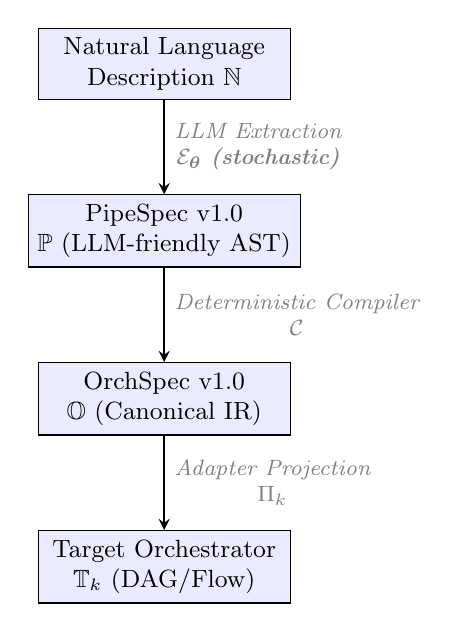
\begin{tikzpicture}[
    node distance=1.2cm and 1.0cm,
    box/.style={rectangle,draw=black,fill=blue!8,minimum width=3.2cm,minimum height=0.8cm,align=center,font=\small},
    arrow/.style={->,>=stealth,thick},
    labelstyle/.style={font=\footnotesize\itshape,text=gray,align=center}
]
\node[box] (NL) {Natural Language\\Description $\nspace$};
\node[box,below=of NL] (PS) {PipeSpec v1.0\\$\pspace$ (LLM-friendly AST)};
\node[box,below=of PS] (OS) {OrchSpec v1.0\\$\ospace$ (Canonical IR)};
\node[box,below=of OS] (TG) {Target Orchestrator\\$\tspacek$ (DAG/Flow)};

\draw[arrow] (NL) -- (PS) node[midway,right,labelstyle] {LLM Extraction\\$\ExtractLLM$ \textbf{(stochastic)}};
\draw[arrow] (PS) -- (OS) node[midway,right,labelstyle] {Deterministic Compiler\\$\Compile$};
\draw[arrow] (OS) -- (TG) node[midway,right,labelstyle] {Adapter Projection\\$\Pi_k$};

\end{tikzpicture}
\end{center}

The contribution of this paper is a formal algebraic treatment of the \textbf{PipeSpec layer}: the extraction function, the document space, the validation and correction machinery, and the feedback loops that make LLM-driven extraction practical.

\begin{remark}[Relationship to OrchSpec]
PipeSpec and OrchSpec form a two-format pipeline. PipeSpec is the \emph{loose AST} (flexible, allows nulls, tolerates LLM variability). OrchSpec is the \emph{canonical IR} (strict, deterministic, machine-validated). The compiler $\Compile : \pspace \to \ospace$ bridges them. This paper focuses on PipeSpec; the companion paper \cite{orchspec-formal} covers OrchSpec.
\end{remark}

% ==========================================================================
\section{Foundational Spaces}
% ==========================================================================

\subsection{Natural Language Space}
\begin{definition}[Natural Language Space $\nspace$]
$\nspace \subseteq \Sigma^*$ is the set of all finite strings over a Unicode alphabet that constitute valid natural language descriptions of data pipelines. An element $n \in \nspace$ is typically a text file describing a pipeline's purpose, components, data flow, and operational requirements.
\end{definition}

\begin{remark}
$\nspace$ is not formally decidable (it depends on human communicative intent), but for our purposes it serves as the domain of the extraction function. In practice, $n$ is a prose description such as ``Fetch campaign data from the Ads API, transform metrics, and send an email report.''
\end{remark}

\subsection{PipeSpec Document Space}
\begin{definition}[PipeSpec Space $\pspace$]
$\pspace \subseteq \jspace$ is the set of all JSON documents that validate against the canonical PipeSpec v1.0 JSON Schema ($\sigma_P$, stored in \texttt{schema/pipespec\_schema\_v1.json}) and satisfy all 7 semantic validation rules. An element $p \in \pspace$ is called a \emph{PipeSpec document}.
\end{definition}

A PipeSpec document $p$ has the following mandatory structure:
\begin{equation}
p =
\begin{cases}
\texttt{pipespec\_version} &: \text{fixed } \texttt{"1.0"} \\
\texttt{metadata}          &: M \quad \text{(provenance)} \\
\texttt{pipeline\_summary} &: S \quad \text{(identity)} \\
\texttt{components}        &: [C_1, \dots, C_m] \quad (m \geq 1) \\
\texttt{flow\_structure}   &: F \quad \text{(topology)} \\
\texttt{parameters}        &: \Psi \quad \text{(5 groups)} \\
\texttt{integrations}      &: I \quad \text{(catalogue + lineage)}
\end{cases}
\end{equation}

with an optional $\texttt{extensions}$ key for non-normative domain-specific data.

\subsection{Key Type Vocabularies}

\begin{definition}[Component Category Vocabulary]
The component taxonomy $\mathcal{T}_C$ consists of 8 categories:
\begin{equation}
\mathcal{T}_C = \{\texttt{Extractor},\; \texttt{Transformer},\; \texttt{Loader},\; \texttt{Reconciliator},\; \texttt{QualityCheck},\; \texttt{Notifier},\; \texttt{Sensor},\; \texttt{Custom}\}
\end{equation}
These categories are designed to be inferable from natural language descriptions (e.g., ``fetch from API'' $\to$ \texttt{Extractor}, ``send email'' $\to$ \texttt{Notifier}).
\end{definition}

\begin{definition}[Executor Type Vocabulary]
The executor type vocabulary $\mathcal{T}_E$ (7 types):
\begin{equation}
\mathcal{T}_E = \{\texttt{python},\; \texttt{http},\; \texttt{sql},\; \texttt{bash},\; \texttt{email},\; \texttt{docker},\; \texttt{custom}\}
\end{equation}
Note that PipeSpec uses a looser vocabulary than OrchSpec (e.g., \texttt{python} vs. \texttt{python\_script} in OrchSpec). The compiler $\Compile$ normalises these during the PipeSpec $\to$ OrchSpec transformation.
\end{definition}

\begin{definition}[Flow Pattern Vocabulary]
The flow pattern vocabulary $\mathcal{T}_F$ (5 patterns):
\begin{equation}
\mathcal{T}_F = \{\texttt{sequential},\; \texttt{parallel},\; \texttt{dag},\; \texttt{conditional},\; \texttt{loop}\}
\end{equation}
\end{definition}

\begin{definition}[IO Kind Vocabulary]
The IO kind vocabulary $\mathcal{T}_K$ (5 kinds):
\begin{equation}
\mathcal{T}_K = \{\texttt{file},\; \texttt{table},\; \texttt{api},\; \texttt{object},\; \texttt{stream}\}
\end{equation}
\end{definition}

\begin{definition}[Integration Type Vocabulary]
The integration type vocabulary $\mathcal{T}_I$ (7 types):
\begin{equation}
\mathcal{T}_I = \{\texttt{api},\; \texttt{database},\; \texttt{filesystem},\; \texttt{object\_store},\; \texttt{message\_queue},\; \texttt{smtp},\; \texttt{other}\}
\end{equation}
\end{definition}

\subsection{Well-Formedness Predicate}
\begin{definition}[PipeSpec Validation]
The predicate $\ValidateP(p)$ for $p \in \jspace$ holds iff:
\begin{equation}
\ValidateP(p) \equiv \ValidateSchemaP(p) \land \ValidateSemanticP(p)
\end{equation}
where $\ValidateSchemaP(p)$ holds iff $p$ validates against $\sigma_P$ (JSON Schema Draft-07), and $\ValidateSemanticP(p)$ holds iff none of the 7 semantic rules raise errors. (In v1, semantic rule violations are \textbf{warnings} that do not affect the binary validity of $p$.)
\end{definition}

\begin{corollary}
$\pspace = \{p \in \jspace \mid \ValidateSchemaP(p)\}$ in v1, since semantic rules are advisory. The semantic-warning subset is $\pspace^{\text{sem}} = \{p \in \pspace \mid \ValidateSemanticP(p)\}$.
\end{corollary}

% ==========================================================================
\section{The LLM as a Stochastic Parser}
% ==========================================================================

The central novelty of PipeSpec is using an LLM as the front-end parser that maps natural language to a structured AST. We formalise this as follows.

\subsection{Extraction Function}
\begin{definition}[Raw Extraction]
Let $\bm\theta \in \Theta$ denote the LLM configuration (model weights, prompt template, temperature, provider). The \emph{raw extraction function} is:
\begin{equation}
\ExtractRaw_{\bm\theta} : \nspace \to \Sigma^*
\end{equation}
which maps a natural language description to a raw string (the LLM's text output). This string may or may not be valid JSON.
\end{definition}

\begin{definition}[Parsing Function]
The parsing function $\ParseLLM : \Sigma^* \to \jspace \cup \{\bot\}$ attempts to extract a JSON object from the LLM's output:
\begin{equation}
\ParseLLM(s) =
\begin{cases}
d \in \jspace & \text{if a valid JSON object can be parsed from } s \\
\bot & \text{otherwise}
\end{cases}
\end{equation}
This includes handling of markdown code fences (\texttt{```json ... ```}), partial JSON extraction, and JSON syntax errors.
\end{definition}

\begin{definition}[Extraction Function]
The full extraction is the composition:
\begin{equation}
\ExtractLLM_{\bm\theta} = \ParseLLM \circ \ExtractRaw_{\bm\theta} : \nspace \to \jspace \cup \{\bot\}
\end{equation}
\end{definition}

\begin{remark}[LLM as a Probabilistic Type-Directed Synthesiser]
The LLM is not a deterministic parser but a \emph{probabilistic type-directed synthesiser}. Given a natural language description $n \in \nspace$ and a type specification $\sigma_P$ (the JSON Schema), the LLM stochastically generates an AST node $p \in \jspace$ that aims to satisfy the type constraints. The prompt includes:
\begin{enumerate}[label=(\roman*),leftmargin=*]
    \item The canonical schema $\sigma_P$ (or its compressed prompt profile $\sigma_P^{\text{prompt}}$);
    \item An example document showing the expected structure;
    \item Enum tables for all restricted vocabularies;
    \item Structural rules (e.g., ``\texttt{flow\_structure.nodes} is an OBJECT, not an array'');
    \item Common mistakes to avoid.
\end{enumerate}
\end{remark}

\subsection{The Prompt Profile as Schema Compression}
\begin{definition}[Prompt Profile]
The \emph{prompt profile} $\sigma_P^{\text{prompt}}$ is a non-normative, dereferenced, size-reduced copy of the canonical schema $\sigma_P$, deterministically generated from $\sigma_P$ by the function:
\begin{equation}
\text{profile} : \sigma_P \mapsto \sigma_P^{\text{prompt}}
\end{equation}
It removes all \texttt{\$ref} indirections, reduces description strings to key points, and omits validation-only constraints (e.g., \texttt{additionalProperties: false}) that are not needed for generation guidance. The profile is \emph{never} used for validation — only the canonical schema $\sigma_P$ is normative.
\end{definition}

\begin{proposition}[Profile Soundness]
Any document that validates against $\sigma_P$ would be structurally admissible under $\sigma_P^{\text{prompt}}$, but not conversely. The profile is a \emph{relaxation} of the schema, not an extension.
\end{proposition}

\subsection{Extraction with Repair}
\begin{definition}[Repair Loop]
PipeSpec implements an \emph{iterative repair loop} that feeds validation errors back to the LLM for correction. Let $\errs(p)$ be the set of schema errors in document $p$. The \emph{single-round repair} is:
\begin{equation}
\RepairLLM_{\bm\theta}(p, n) = \ParseLLM \circ \ExtractRaw_{\bm\theta}\big(\text{repair\_prompt}(p, n, \errs(p))\big)
\end{equation}
where $\text{repair\_prompt}$ constructs a prompt containing the current document, the original description, and the formatted error list.

The full repair loop is an iterated function:
\begin{equation}
p_0 = \ExtractLLM_{\bm\theta}(n), \quad p_{i+1} = \RepairLLM_{\bm\theta}(p_i, n)
\end{equation}
which terminates when $\ValidateSchemaP(p_i)$ holds or a maximum number of attempts $A_{\max}$ (default 4) is reached.
\end{definition}

\begin{proposition}[Temperature Annealing]
The LLM temperature $T_i$ at iteration $i$ follows an annealing schedule:
\begin{equation}
T_i =
\begin{cases}
\min(T_{\text{base}}, 0.05) & i = 0 \\
\min(T_{\text{base}}, 0.15)  & i = 1 \\
\min(T_{\text{base}} + 0.1, 0.4) & i \geq 2
\end{cases}
\end{equation}
Starting cold encourages precise structural output; warming up allows creative repair of stubborn errors.
\end{proposition}

% ==========================================================================
\section{PipeSpec Document Structure}
% ==========================================================================

\subsection{The 7-Section Architecture}
\begin{definition}[PipeSpec as a 7-Tuple]
A PipeSpec document is a typed 7-tuple:
\begin{equation}
p = (v, M, S, \mathbf{C}, F, \Psi, I)
\end{equation}
where each component is defined below.
\end{definition}

\subsubsection{Version}
$v = \texttt{"1.0"}$ — a constant string constraining the schema version.

\subsubsection{Metadata $M$}
\begin{align}
M &=
\begin{cases}
\texttt{analysis\_timestamp} &: \text{ISO 8601 datetime (required)} \\
\texttt{source\_file}        &: \text{string (optional)} \\
\texttt{llm\_provider}       &: \text{string (optional)} \\
\texttt{llm\_model}          &: \text{string (optional)} \\
\texttt{analysis\_results}   &: \text{object (optional)} \\
\texttt{validation\_warnings}&: [\text{string}] \text{(optional)}
\end{cases}
\end{align}

\subsubsection{Pipeline Summary $S$}
\begin{align}
S &=
\begin{cases}
\texttt{name}          &: \text{string (required)} \\
\texttt{description}   &: \text{string (optional)} \\
\texttt{flow\_patterns}&: [\mathcal{T}_F] \text{(required, } \geq 1) \\
\texttt{task\_executors}&: [\mathcal{T}_E] \text{(optional)} \\
\texttt{complexity}    &: \{\texttt{low}, \texttt{medium}, \texttt{high}\} \text{(required)}
\end{cases}
\end{align}

\subsubsection{Components $\mathbf{C}$}
$\mathbf{C} = [C_1, \dots, C_m]$ where $m \geq 1$ and each component $C_i$ is:
\begin{align}
C_i &=
\begin{cases}
\texttt{id}            &: \text{Id (required, pattern } \texttt{\^{}[A-Za-z][A-Za-z0-9\_-]*\$)} \\
\texttt{name}          &: \text{string (required)} \\
\texttt{category}      &: \mathcal{T}_C \text{(required)} \\
\texttt{description}   &: \text{string (optional)} \\
\texttt{executor\_type}&: \mathcal{T}_E \text{(required)} \\
\texttt{executor\_config}&: \text{object | null (optional)} \\
\texttt{io\_spec}      &: [\text{IOSpecItem}] \text{(required, } \geq 1) \\
\texttt{upstream\_policy}&: \text{UpstreamPolicy (optional)} \\
\texttt{retry\_policy}  &: \text{RetryPolicy (optional)} \\
\texttt{concurrency}    &: \text{Concurrency (optional)} \\
\texttt{connections}    &: [\text{ConnectionRef}] \text{(optional)} \\
\texttt{datasets}       &: \text{Datasets (optional)}
\end{cases}
\end{align}

Each IO spec item has:
\begin{align}
\text{IOSpecItem} &=
\begin{cases}
\texttt{name}          &: \text{Id} \\
\texttt{direction}     &: \{\texttt{input}, \texttt{output}\} \\
\texttt{kind}          &: \mathcal{T}_K \\
\texttt{format}        &: \text{string (free-form)} \\
\texttt{path\_pattern}  &: \text{string | null} \\
\texttt{connection\_id} &: \text{Id | null}
\end{cases}
\end{align}

\subsubsection{Flow Structure $F$}
The flow structure uses a \textbf{dual representation}: nodes (a map keyed by node ID) and edges (a list of directed edges). This is a key design decision — nodes carry component binding and policies, while edges carry connectivity and conditions.

\begin{align}
F &=
\begin{cases}
\texttt{pattern}      &: \mathcal{T}_F \text{(required)} \\
\texttt{entry\_points}&: [\text{Id}] \text{(required, } \geq 1) \\
\texttt{nodes}        &: \{\text{Id} \mapsto \text{FlowNode}\} \text{(required)} \\
\texttt{edges}        &: [\text{FlowEdge}] \text{(required)}
\end{cases}
\end{align}

Each flow node binds a component to the topology:
\begin{align}
\text{FlowNode} &=
\begin{cases}
\texttt{kind}              &: \{\texttt{Task}, \texttt{Group}, \texttt{Branch}, \texttt{Sensor}, \texttt{ParallelGroup}\} \\
\texttt{component\_type\_id}&: \text{Id (references a component)} \\
\texttt{upstream\_policy}   &: \text{UpstreamPolicy} \\
\texttt{next\_nodes}        &: [\text{Id}]
\end{cases}
\end{align}

Each edge defines a directed link:
\begin{align}
\text{FlowEdge} &=
\begin{cases}
\texttt{from}      &: \text{Id (refers to a node key)} \\
\texttt{to}        &: \text{Id (refers to a node key)} \\
\texttt{edge\_type}&: \{\texttt{success}, \texttt{failure}, \texttt{always}, \texttt{conditional}\} \\
\texttt{condition} &: \text{string | null} \\
\texttt{metadata}  &: \text{object (optional)}
\end{cases}
\end{align}

\begin{remark}[Dual Representation Rationale]
The dual representation (nodes + edges) separates two concerns: \textbf{node-level} (component binding, upstream policies, parallelism configuration) from \textbf{edge-level} (trigger conditions, branching semantics). This reflects the reality that most orchestrators encode topology in both nodes and edges, and makes the LLM extraction task more natural — components define \emph{what} runs, nodes define \emph{how} they participate in the DAG, and edges define \emph{when} they trigger.
\end{remark}

\subsubsection{Parameters $\Psi$}
Parameters are organised into 5 fixed groups:
\begin{align}
\Psi &=
\begin{cases}
\texttt{pipeline}    &: \text{ParameterGroup} \quad \text{(pipeline-level params)} \\
\texttt{schedule}    &: \text{ParameterGroup} \quad \text{(cron, timezone, etc.)} \\
\texttt{execution}   &: \text{ParameterGroup} \quad \text{(runtime config)} \\
\texttt{components}  &: \{\text{Id} \mapsto \text{ParameterGroup}\} \quad \text{(per-component)} \\
\texttt{environment} &: \{\text{name} \mapsto \text{EnvParamSpec}\} \quad \text{(secrets/env vars)}
\end{cases}
\end{align}

Each parameter spec has:
\begin{align}
\text{ParameterSpec} &=
\begin{cases}
\texttt{description} &: \text{string} \\
\texttt{type}        &: \{\texttt{string}, \texttt{integer}, \texttt{float}, \texttt{boolean}, \texttt{array}, \texttt{object}, \texttt{datetime}\} \\
\texttt{default}     &: \text{any | null} \\
\texttt{required}    &: \text{boolean}
\end{cases}
\end{align}

\begin{remark}[Security Constraint]
PipeSpec documents MUST NOT contain actual secret values. Environment parameters that represent secrets (API keys, connection strings) must have $\texttt{default} = \texttt{null}$ and $\texttt{required} = \texttt{true}$. The actual values are resolved at runtime by the target orchestrator's secret backend.
\end{remark}

\subsubsection{Integrations $I$}
The integrations section has two parts — a connection catalogue and a data lineage declaration:
\begin{align}
I &=
\begin{cases}
\texttt{connections}   &: [\text{IntegrationConnection}] \\
\texttt{data\_lineage} &: \text{DataLineage}
\end{cases}
\end{align}

Each connection:
\begin{align}
\text{IntegrationConnection} &=
\begin{cases}
\texttt{id}                 &: \text{Id} \\
\texttt{name}               &: \text{string} \\
\texttt{type}               &: \mathcal{T}_I \\
\texttt{config}             &: \text{object (free-form)} \\
\texttt{authentication}     &: \text{object (free-form, references secrets by name)} \\
\texttt{used\_by\_components}&: [\text{Id}] \\
\texttt{direction}          &: \{\texttt{input}, \texttt{output}, \texttt{both}\}
\end{cases}
\end{align}

The data lineage captures coarse data flow:
\begin{align}
\text{DataLineage} &=
\begin{cases}
\texttt{sources}               &: [\text{string}] \quad \text{(upstream data sources)} \\
\texttt{sinks}                 &: [\text{string}] \quad \text{(downstream destinations)} \\
\texttt{intermediate\_datasets}&: [\text{string}] \quad \text{(intermediate artefacts)}
\end{cases}
\end{align}

% ==========================================================================
\section{Validation Formalism}
% ==========================================================================

PipeSpec validation is two-layered: schema validation (structural) and semantic validation (graph/cross-reference integrity).

\subsection{Schema Validation}
\begin{definition}[Schema Validation Function]
$\ValidateSchemaP : \jspace \to \{\top, \bot\} \times \errs$ validates a JSON object against $\sigma_P$. It returns $(\top, \emptyset)$ iff the document satisfies all structural constraints (required fields, enum values, type matches, pattern constraints, \texttt{additionalProperties: false}). Otherwise it returns $(\bot, E)$ where $E$ is a non-empty set of schema violations, each with a JSON Pointer \texttt{instance\_path} and a human-readable \texttt{message}.
\end{definition}

\subsection{Semantic Validation}
\begin{definition}[Semantic Validation Function]
$\ValidateSemanticP : \jspace \to \warns$ runs 7 graph-theoretic and cross-reference integrity rules. In v1, these rules emit \textbf{warnings} only — they do not affect the binary validity of $p$.
\end{definition}

\subsubsection{The 7 Semantic Rules}

\begin{definition}[PIPESPEC-SEM-01 — Duplicate Component IDs]
$\forall\, i \neq j:\; \texttt{id}(C_i) \neq \texttt{id}(C_j)$. Duplicate component IDs cause ambiguity in flow references and are flagged.
\end{definition}

\begin{definition}[PIPESPEC-SEM-02 — Integration Reference Resolution]
For any $\texttt{io\_spec}[k].\texttt{connection\_id}$ that is non-null, the value must exist in $\texttt{integrations.connections}[*].\texttt{id}$. Similarly for $\texttt{connections}[*].\texttt{id}$ on components.
\end{definition}

\begin{definition}[PIPESPEC-SEM-03 — Flow Cross-Reference Resolution]
Every entry point must be a key in $\texttt{flow\_structure.nodes}$. Every edge's $\texttt{from}$ and $\texttt{to}$ must be keys in $\texttt{flow\_structure.nodes}$.
\end{definition}

\begin{definition}[PIPESPEC-SEM-04 — Node-Component Binding]
Every $\texttt{flow\_structure.nodes}[k].\texttt{component\_type\_id}$ must exist among $\texttt{components}[*].\texttt{id}$.
\end{definition}

\begin{definition}[PIPESPEC-SEM-05 — Self-Loops and Duplicate Edges]
An edge with $\texttt{from} = \texttt{to}$ is a self-loop (unusual for DAG pipelines). Duplicate edges (same $\texttt{from}, \texttt{to}, \texttt{edge\_type}, \texttt{condition}$) are redundant. Both are flagged as warnings.
\end{definition}

\begin{definition}[PIPESPEC-SEM-06 — Cycle Detection (DAG Constraint)]
Let $\texttt{pattern} \neq \texttt{loop}$. Construct the directed graph $G = (V, E)$ where $V = \text{keys}(\texttt{nodes})$ and $E = \{(\texttt{from}, \texttt{to}) \mid \text{edge} \in \texttt{edges}\}$. $G$ must be acyclic. If a cycle is detected, the warning suggests either removing the cycle or setting $\texttt{pattern} = \texttt{loop}$.
\end{definition}

\begin{definition}[PIPESPEC-SEM-07 — Reachability and Entry Point Sanity]
Every node in $\texttt{nodes}$ must be reachable by directed traversal from at least one entry point. Entry points should have in-degree 0 (if an entry point has incoming edges, it's flagged as suspicious).
\end{definition}

\subsection{Graph-Theoretic Model of Flow Structure}
\begin{definition}[PipeSpec Flow Graph]
The flow structure $F$ induces a typed directed graph $G_F = (V, E, \lambda_V, \lambda_E)$ where:
\begin{itemize}[leftmargin=*]
    \item $V = \text{keys}(\texttt{nodes})$ — the set of node identifiers.
    \item $E = \{(\texttt{from}, \texttt{to}) \mid \text{edge} \in \texttt{edges}\}$ — the set of directed edges.
    \item $\lambda_V : V \to \texttt{component\_type\_id} \times \texttt{kind} \times \texttt{upstream\_policy}$ — node labels.
    \item $\lambda_E : E \to \{\texttt{success}, \texttt{failure}, \texttt{always}, \texttt{conditional}\} \times \text{cond}$ — edge labels.
\end{itemize}
\end{definition}

The 7 semantic rules can be expressed as predicates on $G_F$:
\begin{align}
\text{SEM-01} &: \text{injective}(\texttt{id} : \mathbf{C} \to \text{string}) \\
\text{SEM-02} &: \forall\, \text{ref} \in \text{io\_connections} \cup \text{component\_connections}:\; \text{ref} \in \text{integration\_ids} \\
\text{SEM-03} &: \texttt{entry\_points} \subseteq V \;\land\; \forall\, e \in E:\; e.\texttt{from} \in V \land e.\texttt{to} \in V \\
\text{SEM-04} &: \forall\, v \in V:\; \lambda_V(v).\texttt{component\_type\_id} \in \{\texttt{id}(c) \mid c \in \mathbf{C}\} \\
\text{SEM-05} &: \nexists\, e \in E:\; e.\texttt{from} = e.\texttt{to} \;\land\; E \text{ has no duplicates} \\
\text{SEM-06} &: \texttt{pattern} \neq \texttt{loop} \;\Longrightarrow\; G_F \text{ is acyclic} \\
\text{SEM-07} &: \text{Reach}(\texttt{entry\_points}) = V \;\land\; \forall\, ep \in \texttt{entry\_points}:\; \deg^-(ep) = 0
\end{align}

% ==========================================================================
\section{The Correction Model: Autofix and LLM Repair}
% ==========================================================================

PipeSpec provides two correction mechanisms: a deterministic autofix engine and an LLM-assisted repair loop. Together they form a \textbf{contraction mapping} on the error space.

\subsection{Deterministic Autofix}
\begin{definition}[Autofix Function]
$\Autofix : \jspace \to \jspace \times \fixs$ is a deterministic, safe, single-round fix function. It applies structural corrections that are inferable from the document's own structure without inventing domain content.
\end{definition}

\begin{definition}[Fix Action Space]
$\fixs$ is the set of fix actions. Each action has a stable code from:
\begin{align}
\mathcal{F}_{\text{codes}} = \{\; &\text{FIX-TOP-01}, \dots, \text{FIX-TOP-04}, \\
&\text{FIX-COMP-01}, \dots, \text{FIX-COMP-04}, \\
&\text{FIX-FLOW-01}, \dots, \text{FIX-FLOW-07}, \\
&\text{FIX-PARAM-01}, \text{FIX-INTEG-01} \;\}
\end{align}
\end{definition}

\begin{theorem}[Autofix Safety]
$\Autofix(p)$ never removes or alters user-supplied semantic content. It only:
\begin{enumerate}[label=(\alph*),leftmargin=*]
    \item Adds missing structural defaults (e.g., empty $\texttt{parameters}$ block);
    \item Converts type errors where the intent is unambiguous (e.g., $\texttt{components}$ dict $\to$ array);
    \item Normalises known aliases (e.g., $\texttt{SQLTransform} \to \texttt{Transformer}$, $\texttt{python\_callable} \to \texttt{python}$);
    \item Injects structural placeholders (e.g., stub $\texttt{io\_spec}$ marked for review);
    \item Removes dangling cross-references (entry points / edges pointing to non-existent nodes);
    \item Stubs missing Task nodes for known components.
\end{enumerate}
\end{theorem}

\subsection{Iterative Autofix}
\begin{definition}[Multi-Round Autofix]
$\AutofixMulti : \jspace \to \jspace \times \fixs \times \mathbb{N}$ iterates $\Autofix$ until convergence:
\begin{equation}
\AutofixMulti(p) = \Autofix^n(p) \quad \text{where } n = \min\{k \mid \Autofix^{k}(p) = \Autofix^{k-1}(p)\}
\end{equation}
with a hard cap of $\text{MAX\_ROUNDS} = 5$. Convergence is detected when no new fix actions are produced or the schema error count stops decreasing.
\end{definition}

\subsection{LLM-Assisted Repair}
\begin{definition}[LLM Repair Function]
When deterministic autofix cannot resolve all errors (content gaps requiring domain knowledge), the system escalates to LLM repair. Given the best-effort autofixed document $p_{\text{auto}}$ and the original natural language description $n$:
\begin{equation}
p_{\text{repaired}} = \RepairLLM_{\bm\theta}(p_{\text{auto}}, n)
\end{equation}
This constructs a prompt containing: the current document, the original description text, and a compact error summary. The LLM returns a corrected JSON object. This is iterated up to 3 attempts.
\end{definition}

\subsection{Contraction Mapping Property}
\begin{proposition}[Error Contraction]
Let $e(p) = |\errs(p)|$ be the error count for document $p$. For the composition of autofix and LLM repair:
\begin{equation}
e(\RepairLLM_{\bm\theta}(\AutofixMulti(p), n)) \leq e(p)
\end{equation}
and typically $e$ is strictly decreasing. Empirically, the repair loop converges to $e = 0$ within 3--4 iterations for well-formed natural language descriptions.
\end{proposition}

\begin{proof}[Sketch]
$\AutofixMulti$ is purely subtractive on errors (it fixes structural issues without introducing new ones). $\RepairLLM_{\bm\theta}$ receives the exact error list and is prompted to fix only those errors. Since the LLM has access to the original description, it can fill content gaps. Each iteration reduces or maintains the error count. The process is bounded by the attempt limit.
\end{proof}

% ==========================================================================
\section{The Hints System}
% ==========================================================================

The hints system translates validation errors into actionable, tiered guidance.

\begin{definition}[Hint Space]
$\hintspace$ is the set of hints. A hint is a tuple:
\begin{equation}
h = (\texttt{code}, \texttt{tier}, \texttt{severity}, \texttt{message}, \texttt{paths}, \texttt{suggested\_action})
\end{equation}
where $\texttt{tier} \in \{\texttt{structural}, \texttt{content}, \texttt{semantic}\}$ and $\texttt{severity} \in \{\texttt{low}, \texttt{medium}, \texttt{high}\}$.
\end{definition}

\begin{definition}[Hint Generation Function]
$\Hints : \errs \times \warns \to \mathcal{P}(\hintspace)$ is a deterministic function that maps schema errors and semantic warnings to a deduplicated, severity-sorted set of hints.
\end{definition}

\begin{proposition}[LLM Escalation Detection]
The predicate $\texttt{llm\_escalation\_needed} : \mathcal{P}(\hintspace) \to \{\top, \bot\}$ returns $\top$ iff any hint has $\texttt{tier} = \texttt{content}$ and $\texttt{severity} = \texttt{high}$ (i.e., the gap requires domain knowledge to fill).
\end{proposition}

The two-tier classification is central to the correction workflow:

\begin{table}[htbp]
\centering
\caption{Hint tier classification.}
\label{tab:hints}
\begin{tabular}{@{}lll@{}}
\toprule
\textbf{Tier} & \textbf{Resolution} & \textbf{Example} \\
\midrule
\texttt{structural} & Deterministic autofix can stub & Missing $\texttt{parameters}$ block \\
\texttt{content}    & Requires LLM / domain knowledge & Missing component $\texttt{category}$ \\
\texttt{semantic}   & Graph-theoretic issue  & Cycle in DAG, unreachable node \\
\bottomrule
\end{tabular}
\end{table}

% ==========================================================================
\section{Semantic Diff Formalism}
% ==========================================================================

\begin{definition}[Semantic Diff Function]
$\DiffP : \pspace \times \pspace \to \dspace$ compares two PipeSpec documents at the meaning level (not raw text), producing a structured diff report.
\end{definition}

The diff compares:
\begin{enumerate}[label=(\alph*),leftmargin=*]
    \item \textbf{Pipeline summary}: name, description, flow patterns, task executors, complexity.
    \item \textbf{Components}: by stable $\texttt{id}$ — additions, removals, field-level changes (category, executor\_type, io\_spec, retry\_policy, connections).
    \item \textbf{Flow nodes}: additions and removals of node IDs.
    \item \textbf{Flow edges}: treated as a set of $(\texttt{from}, \texttt{to}, \texttt{edge\_type}, \texttt{condition})$ tuples.
    \item \textbf{Integrations}: by stable $\texttt{id}$ — additions, removals, field changes.
    \item \textbf{Parameter keys}: flattened paths compared as sets.
\end{enumerate}

\begin{definition}[Component Projection for Diff]
To avoid comparing irrelevant fields, each component is projected to a canonical comparison form:
\begin{align}
\pi_{\text{diff}}(C) &= (\texttt{name}, \texttt{category}, \texttt{executor\_type}, \texttt{io\_spec}, \\
&\quad\; \texttt{upstream\_policy}, \texttt{retry\_policy}, \texttt{concurrency}, \texttt{datasets}, \texttt{connections})
\end{align}
\end{definition}

\begin{proposition}[Set-Theoretic Diff Completeness]
$\DiffP(p_1, p_2)$ captures all structural differences between $p_1$ and $p_2$ that are semantically meaningful for pipeline execution. Metadata-only changes (timestamps, LLM model names) are excluded from the diff.
\end{proposition}

% ==========================================================================
\section{Relationship to OrchSpec}
% ==========================================================================

\begin{definition}[The Compiler Bridge]
The deterministic compiler $\Compile : \pspace \to \ospace$ (defined in the companion paper \cite{orchspec-formal}) maps PipeSpec documents to OrchSpec canonical IR documents. The relationship between the two spaces is:
\begin{equation}
\text{PipeSpec} \xrightarrow{\Compile} \text{OrchSpec}
\end{equation}
where $\Compile$ is a deterministic, label-normalising graph isomorphism on the DAG topology (component identifiers are canonicalised, executor types are mapped via $\tau_E$, and semantic content is preserved).
\end{definition}

\begin{theorem}[End-to-End Pipeline]
The complete pipeline from natural language to a target orchestrator is:
\begin{equation}
\text{Pipeline}_k = \Pi_k \circ \Compile \circ \ExtractLLM_{\bm\theta} : \nspace \to \tspacek \cup \{\bot, \uparrow\}
\end{equation}
A full formal treatment of OrchSpec — including the compiler $\Compile$ as a graph homomorphism, the 21 semantic validation rules, and the adapter projection functors $\Pi_k$ — is given in the companion paper~\cite{orchspec-formal}. The unified OPOS meta-specification~\cite{opos-formal} provides the combined formal framework covering both layers, conformance criteria, and the OTS (Open Transformation Specification) bridge.
\end{theorem}

\begin{corollary}[Separation of Concerns]
\begin{enumerate}[label=(\roman*),leftmargin=*]
    \item The LLM deals only with \textbf{understanding} (NL $\to$ PipeSpec).
    \item The compiler deals only with \textbf{normalising} (PipeSpec $\to$ OrchSpec).
    \item The adapter deals only with \textbf{projecting} (OrchSpec $\to$ target).
\end{enumerate}
Each stage can be developed, tested, and versioned independently. This separation is the architectural foundation of the entire OrchSpec ecosystem.
\end{corollary}

% ==========================================================================
\section{Extensibility}
% ==========================================================================

\subsection{Extending the Schema}
\begin{definition}[Extension Point]
The $\texttt{extensions}$ key at the top level (and on components) is an \texttt{additionalProperties: true} object that serves as the primary extension mechanism. Organisations can add domain-specific fields (e.g., compliance metadata, cost centre) without modifying the canonical schema.
\end{definition}

\subsection{Adding a New Semantic Rule}
\begin{definition}[Semantic Rule Registration]
A new rule $\text{PIPESPEC-SEM-}i$ (for $i > 7$) is a function $r_i : \jspace \to \warns$ registered in the $\texttt{SEMANTIC\_RULES}$ list. New rules are additive and must be:
\begin{enumerate}[label=(\alph*),leftmargin=*]
    \item Deterministic;
    \item Side-effect free;
    \item Non-crashing (exceptions are caught and converted to semantic warnings).
\end{enumerate}
\end{definition}

\subsection{Adding a New Autofix Rule}
\begin{definition}[Autofix Rule Registration]
A new fix with code $\text{FIX-}\langle\text{CAT}\rangle\text{-}NN$ is added to the autofix engine. It must be:
\begin{enumerate}[label=(\alph*),leftmargin=*]
    \item \textbf{SAFE}: only fix what can be inferred from the document's own structure;
    \item \textbf{AUDITABLE}: every action is recorded as a $\texttt{FixAction}$;
    \item \textbf{CONSERVATIVE}: never invent domain content.
\end{enumerate}
\end{definition}

\subsection{Adding a New LLM Provider}
\begin{definition}[Provider Abstraction]
The LLM runtime abstracts over providers via a unified interface $\texttt{call\_llm\_json}(\texttt{config}, \texttt{system\_prompt}, \texttt{user\_prompt}) \to \Sigma^*$. Adding a new provider requires:
\begin{enumerate}[label=(\alph*),leftmargin=*]
    \item A default base URL and model in the provider registry;
    \item API key resolution logic (environment variable priority list);
    \item A client call implementation (OpenAI-compatible or native SDK).
\end{enumerate}
\end{definition}

% ==========================================================================
\section{Discussion}
% ==========================================================================

\subsection{Why a Dual Node/Edge Representation?}
The PipeSpec flow structure uses both $\texttt{nodes}$ (an object map) and $\texttt{edges}$ (an array). This dual representation is deliberate:
\begin{itemize}[leftmargin=*]
    \item \textbf{Nodes} carry \emph{component binding} — which component runs, what its upstream policy is, what its next nodes are. This mirrors how orchestrators like Airflow define tasks with their properties.
    \item \textbf{Edges} carry \emph{trigger semantics} — success/failure/conditional triggers, with optional condition expressions. This mirrors how orchestrators define dependencies.
\end{itemize}
The LLM is instructed to produce both, and the validator checks cross-consistency (SEM-03, SEM-04). This redundancy improves extraction accuracy because each representation reinforces the other.

\subsection{Why Semantic Rules Are Warnings in v1}
In PipeSpec v1, semantic rule violations do not cause validation failure ($\texttt{ok} = \texttt{False}$). This is intentional: PipeSpec is designed for LLM extraction, and LLMs frequently produce structurally valid but semantically imperfect documents. By keeping semantic rules as warnings, the system always produces a \emph{best-effort document} that can still be compiled to OrchSpec (which applies its own strict semantic validation). Downstream consumers can opt into stricter enforcement by treating warnings as errors.

\subsection{Why the Prompt Profile Is Non-Normative}
The prompt profile $\sigma_P^{\text{prompt}}$ is a compressed, dereferenced copy of $\sigma_P$ used only in LLM prompts. It is never used for validation. This separation ensures:
\begin{itemize}[leftmargin=*]
    \item The canonical schema $\sigma_P$ remains the single source of truth for validation.
    \item The prompt profile can be optimised for LLM context windows independently of the schema's validation needs.
    \item Changes to the prompt profile (e.g., rewording descriptions for LLM clarity) do not affect what constitutes a valid PipeSpec document.
\end{itemize}

\subsection{Limitations and Future Work}
\begin{itemize}[leftmargin=*]
    \item The extraction function $\ExtractLLM_{\bm\theta}$ is only constrained structurally (JSON Schema), not semantically (pipeline correctness). Future work could explore constrained decoding with semantic constraints.
    \item The semantic rules are limited to graph-theoretic checks (DAG, reachability). Runtime semantic checks (e.g., type compatibility of connected I/O) are deferred to OrchSpec.
    \item The autofix engine is conservative by design. More aggressive fixes (e.g., inferring missing categories from executor types) could be explored but risk introducing errors.
    \item The dual representation (nodes + edges) creates a maintenance burden — changes to components require coordinated updates to nodes. A future version could auto-generate nodes from components and edges.
\end{itemize}

% ==========================================================================
\section{Conclusion}
% ==========================================================================

We have presented a rigorous formal method for PipeSpec, the LLM-friendly extraction format that serves as the front-end of the OrchSpec pipeline ecosystem. The key contributions are:

\begin{enumerate}[label={(\arabic*)}]
    \item \textbf{Algebraic spaces} $\nspace$, $\pspace$ with well-defined membership predicates based on JSON Schema Draft-07.
    \item \textbf{A stochastic parser model} $\ExtractLLM_{\bm\theta} : \nspace \to \pspace \cup \{\bot\}$ where the LLM acts as a probabilistic type-directed synthesiser constrained by $\sigma_P$.
    \item \textbf{A prompt profile} $\sigma_P^{\text{prompt}}$ as a sound relaxation of $\sigma_P$ optimised for LLM context windows.
    \item \textbf{A two-layer validator} $\ValidateP = \ValidateSchemaP \land \ValidateSemanticP$ with 7 graph-theoretic semantic rules formalised as predicates on the flow DAG $G_F$.
    \item \textbf{A correction model} combining deterministic autofix $\AutofixMulti$ (safe, structural) with LLM repair $\RepairLLM_{\bm\theta}$ (content-aware), forming a contraction mapping on error space.
    \item \textbf{A hints system} $\Hints : \errs \times \warns \to \mathcal{P}(\hintspace)$ that translates raw errors into tiered, actionable guidance.
    \item \textbf{A semantic diff} $\DiffP$ that compares PipeSpec documents at the meaning level.
    \item \textbf{Formalisation of the dual representation} (nodes + edges) as a typed directed graph $G_F = (V, E, \lambda_V, \lambda_E)$.
    \item \textbf{Clarification of the PipeSpec–OrchSpec relationship} as a compiler chain $\Compile : \pspace \to \ospace$.
\end{enumerate}

This formalisation provides a foundation for rigorous reasoning about LLM-assisted pipeline extraction and serves as a reference for extending PipeSpec to new domains, new LLM providers, and new correction strategies.

\begin{thebibliography}{9}

\bibitem{orchspec-formal}
A.~Alidu, \emph{A Formal Method for OrchSpec: An Algebraic Framework for Orchestration-Agnostic Pipeline Specification}, 2026.

\bibitem{opos-formal}
A.~Alidu, \emph{OPOS: A Formal Method for the Open Pipeline Orchestration Specification --- Unifying PipeSpec and OrchSpec}, 2026.

\bibitem{pipespec-schema}
PipeSpec Project, \emph{PipeSpec v1 JSON Schema}, \texttt{schema/pipespec\_schema\_v1.json}, 2026.

\bibitem{jsonschema}
A.~Wright, H.~Andrews, \emph{JSON Schema: A Media Type for Describing JSON Documents}, draft-07, 2018.

\end{thebibliography}

\appendix
\section{Notation Glossary}

\begin{table}[htbp]
\centering
\caption{Symbols used in this paper.}
\begin{tabular}{@{}ll@{}}
\toprule
\textbf{Symbol} & \textbf{Meaning} \\
\midrule
$\nspace$          & Natural language description space \\
$\pspace$          & PipeSpec document space \\
$\ospace$          & OrchSpec document space (see companion paper) \\
$\tspacek$         & Target orchestrator-$k$ output space \\
$\ExtractLLM_{\bm\theta}$ & LLM extraction function (stochastic parser) \\
$\ParseLLM$        & JSON parsing function from raw LLM output \\
$\ValidateP$       & Combined PipeSpec validation \\
$\ValidateSchemaP$ & Schema validation against $\sigma_P$ \\
$\ValidateSemanticP$ & Semantic validation (7 rules) \\
$\Autofix$         & Single-round deterministic autofix \\
$\AutofixMulti$    & Multi-round iterative autofix \\
$\RepairLLM_{\bm\theta}$ & LLM-assisted repair function \\
$\DiffP$           & PipeSpec semantic diff \\
$\Hints$           & Hint generation from errors \\
$\Compile$         & PipeSpec $\to$ OrchSpec compiler \\
$\sigma_P$         & Canonical PipeSpec JSON Schema \\
$\sigma_P^{\text{prompt}}$ & Prompt profile (non-normative) \\
$\mathcal{T}_C$    & Component category vocabulary (8 categories) \\
$\mathcal{T}_E$    & Executor type vocabulary (7 types) \\
$\mathcal{T}_F$    & Flow pattern vocabulary (5 patterns) \\
$\mathcal{T}_K$    & IO kind vocabulary (5 kinds) \\
$\mathcal{T}_I$    & Integration type vocabulary (7 types) \\
$G_F = (V, E)$    & Flow DAG induced by $\texttt{flow\_structure}$ \\
\bottomrule
\end{tabular}
\end{table}

\section{Complete Error and Fix Code Taxonomy}

\subsection{Compilation Error Codes (Schema Violations)}
\begin{table}[htbp]
\centering
\caption{Schema validation error patterns in PipeSpec.}
\begin{tabular}{@{}ll@{}}
\toprule
\textbf{Pattern} & \textbf{Meaning} \\
\midrule
\texttt{is a required property} & Missing required field at a given path \\
\texttt{is not of type 'array'} & Type mismatch (e.g., components is an object) \\
\texttt{is not one of}         & Invalid enum value \\
\texttt{should be non-empty}   & Empty required array \\
\texttt{does not match pattern}& Invalid identifier format \\
\bottomrule
\end{tabular}
\end{table}

\subsection{Autofix Codes}
\begin{table}[htbp]
\centering
\caption{Deterministic autofix code taxonomy.}
\begin{tabular}{@{}ll@{}}
\toprule
\textbf{Code} & \textbf{Action} \\
\midrule
FIX-TOP-01 & Add missing \texttt{pipespec\_version} \\
FIX-TOP-02 & Add missing \texttt{parameters} block \\
FIX-TOP-03 & Add missing \texttt{integrations} block \\
FIX-TOP-04 & Add missing \texttt{flow\_structure} block \\
FIX-COMP-01 & Convert \texttt{components} dict $\to$ array \\
FIX-COMP-02 & Add missing \texttt{components} as empty array \\
FIX-COMP-03 & Normalise category/executor aliases \\
FIX-COMP-04 & Inject stub \texttt{io\_spec} placeholder \\
FIX-FLOW-01 & Convert \texttt{nodes} array $\to$ object \\
FIX-FLOW-02 & Add missing \texttt{nodes} as empty map \\
FIX-FLOW-03 & Add missing \texttt{edges} as empty array \\
FIX-FLOW-04 & Add missing \texttt{entry\_points} as empty array \\
FIX-FLOW-05 & Add missing \texttt{pattern} (default \texttt{sequential}) \\
FIX-FLOW-06 & Remove dangling entry points / edge endpoints \\
FIX-FLOW-07 & Stub missing Task nodes for known components \\
FIX-PARAM-01 & Add missing parameter sub-keys \\
FIX-INTEG-01 & Add missing integration sub-keys \\
\bottomrule
\end{tabular}
\end{table}

\end{document}
